\documentclass{standalone}
\usepackage{pgfplots}
\pgfplotsset{compat=newest}
\usetikzlibrary{decorations.markings}
\tikzset{->-/.style={decoration={
  markings,
  mark=at position #1 with {\arrow{>}}},postaction={decorate}}}
  \tikzset{-<-/.style={decoration={
  markings,
  mark=at position #1 with {\arrow{<}}},postaction={decorate}}}
\begin{document}
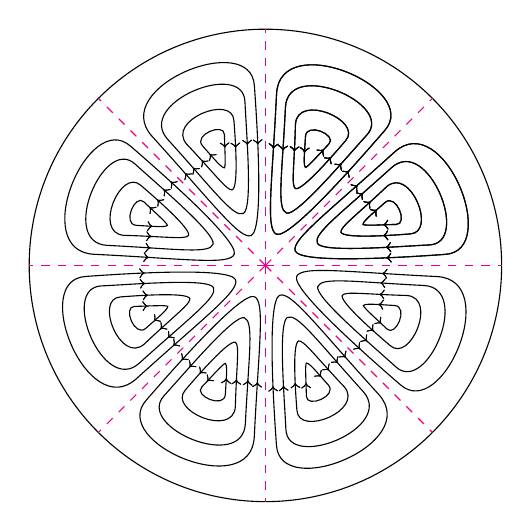
\begin{tikzpicture}[scale=2]

% \path (180:1.5) coordinate (a);
% \path (0:1.5) coordinate (b);
% \foreach \phi in {-30,0,...,30}{
%   \draw[dashed] (a) to[out={\phi},in={180-\phi}] (b);
% }
% \foreach \phi in {60,-60}{
%   \draw[dashed] (a) .. controls ++(\phi:1.5) and ++({180-\phi}:1.5) .. (b);
% }
% \draw[draw=none, fill=white] (a) circle (0.32cm);
% \draw[draw=none, fill=white] (b) circle (0.32cm);

\draw (0,0) circle (1.5cm);

% \foreach \r in {0.3,0.5,0.6,0.7,0.8,1,1.3}{
%   \draw[black,thick,-<-=0.35] (0,0) circle (\r cm);
% }

\foreach \phi in {45,90,...,360}{
  \draw[magenta,dashed] (\phi:0) -- (\phi:1.5);
%   \path (\phi:1.5) coordinate (A);
%   \path  ({180+(180-\phi)}:1.5) coordinate (B);
%   % \draw  to[, in=0];
%   \draw[-<-=0.45,thick] (A) to[out={\phi-180},in=-{\phi-180}] (B);
}

\foreach \phi in {0,90,...,360}{
\begin{scope}[scale=1, rotate=\phi]
\draw[->-=0.2, ->-=0.8] (0.19,0.09) .. controls (0.16,0.16) and (0.39,0.33) .. (0.82,0.72) .. controls (1.13,1.00) and (1.50,0.09) .. (1.14,0.07) .. controls (0.86,0.05) and (0.23,0.01) .. (0.19,0.09) -- cycle;
\draw[->-=0.2, ->-=0.8] (0.33,0.14) .. controls (0.30,0.20) and (0.48,0.33) .. (0.80,0.62) .. controls (1.03,0.83) and (1.31,0.14) .. (1.04,0.13) .. controls (0.83,0.12) and (0.36,0.08) .. (0.33,0.14) -- cycle;
\draw[->-=0.2, ->-=0.8] (0.48,0.21) .. controls (0.47,0.24) and (0.58,0.32) .. (0.77,0.50) .. controls (0.92,0.63) and (1.09,0.21) .. (0.92,0.20) .. controls (0.79,0.19) and (0.50,0.17) .. (0.48,0.21) -- cycle;
\draw[->-=0.2, ->-=0.8] (0.62,0.26) .. controls (0.62,0.28) and (0.67,0.32) .. (0.76,0.40) .. controls (0.83,0.46) and (0.91,0.26) .. (0.83,0.26) .. controls (0.77,0.26) and (0.63,0.25) .. (0.62,0.26) -- cycle;
\end{scope}
}

\foreach \phi in {0,90,...,360}{
\begin{scope}[scale=1, rotate={\phi+45}]
\draw[-<-=0.2, -<-=0.8] (0.19,0.09) .. controls (0.16,0.16) and (0.39,0.33) .. (0.82,0.72) .. controls (1.13,1.00) and (1.50,0.09) .. (1.14,0.07) .. controls (0.86,0.05) and (0.23,0.01) .. (0.19,0.09) -- cycle;
\draw[-<-=0.2, -<-=0.8] (0.33,0.14) .. controls (0.30,0.20) and (0.48,0.33) .. (0.80,0.62) .. controls (1.03,0.83) and (1.31,0.14) .. (1.04,0.13) .. controls (0.83,0.12) and (0.36,0.08) .. (0.33,0.14) -- cycle;
\draw[-<-=0.2, -<-=0.8] (0.48,0.21) .. controls (0.47,0.24) and (0.58,0.32) .. (0.77,0.50) .. controls (0.92,0.63) and (1.09,0.21) .. (0.92,0.20) .. controls (0.79,0.19) and (0.50,0.17) .. (0.48,0.21) -- cycle;
\draw[-<-=0.2, -<-=0.8] (0.62,0.26) .. controls (0.62,0.28) and (0.67,0.32) .. (0.76,0.40) .. controls (0.83,0.46) and (0.91,0.26) .. (0.83,0.26) .. controls (0.77,0.26) and (0.63,0.25) .. (0.62,0.26) -- cycle;
\end{scope}
}
%   \path (\phi:1.5) coordinate (A);
%   \path  ({180+(180-\phi)}:1.5) coordinate (B);
%   % \draw  to[, in=0];
%   \draw[draw=none,fill=white] (A) to[out={\phi-180},in=-{\phi-180}] (B) -- cycle;
% }

\end{tikzpicture}
\end{document}
